\section*{Dati e risultati}

Per ogni resistenza a nostra disposizione abbiamo effettuato una misura volt-amperometrica con entrambi i circuiti realizzati. Pertanto per ognuna delle resistenze abbiamo due coppie di valori di corrente e tensione $(I\ped{x}, V\ped{x})$.
Quindi grazie ai valori acquisiti possiamo determinare il valore sperimentale delle resistenze, sempre sfruttando la legge integrale di Ohm, poichè le resistenze sono componenti circuitali Ohmici.

\begin{equation}
	\text{Amperomero a monte:} \qquad R\ped{x} \,=\, \frac{V\,R\ped{v}}{R\ped{v}\,I\,-\,V}
\end{equation}
\begin{equation}
	\text{Amperomero a valle:} \qquad R\ped{x} \,=\, \frac{V\,-\,I\,R{a}}{I\ped{a}}
\end{equation}
%
dove $R\ped{x}$ indica il valore della resistenza da stimare, $V$ è la differenza di potenziale misurata con il voltometro, $R\ped{v}$ è la resistenza interna del voltometro, $R\ped{a}$ è la resistenza interna dell'amperometro e $I$ è il valore di corrente misurato grazie all'amperometro.

Inoltre per avere un riscontro che i dati ottenuti siano affidabili abbiamo misurato il valore delle varie resistenze mediante il multimetro digitale. In questo modo potremo osservare se ci sono delle discrepanze rilevanti tra il valore teorico e quello sperimentale delle resistenze. Di seguito sono tabulati i risultati ottenuti.

[TABELLA]

Infine abbiamo misurato il valore della resistenza di una lampadina, in grado di sopportate una differenza di potenziale massima di $12\,\si{\volt}$, prendendo una serie di misure volt-amperometriche utilizzando entrambi i circuiti a nostra disposizione.
Anche in questo caso abbiamo graficato i dati e abbiamo ottenuto il seguente risultato:

\begin{figure}[hbtp]
        \centering
        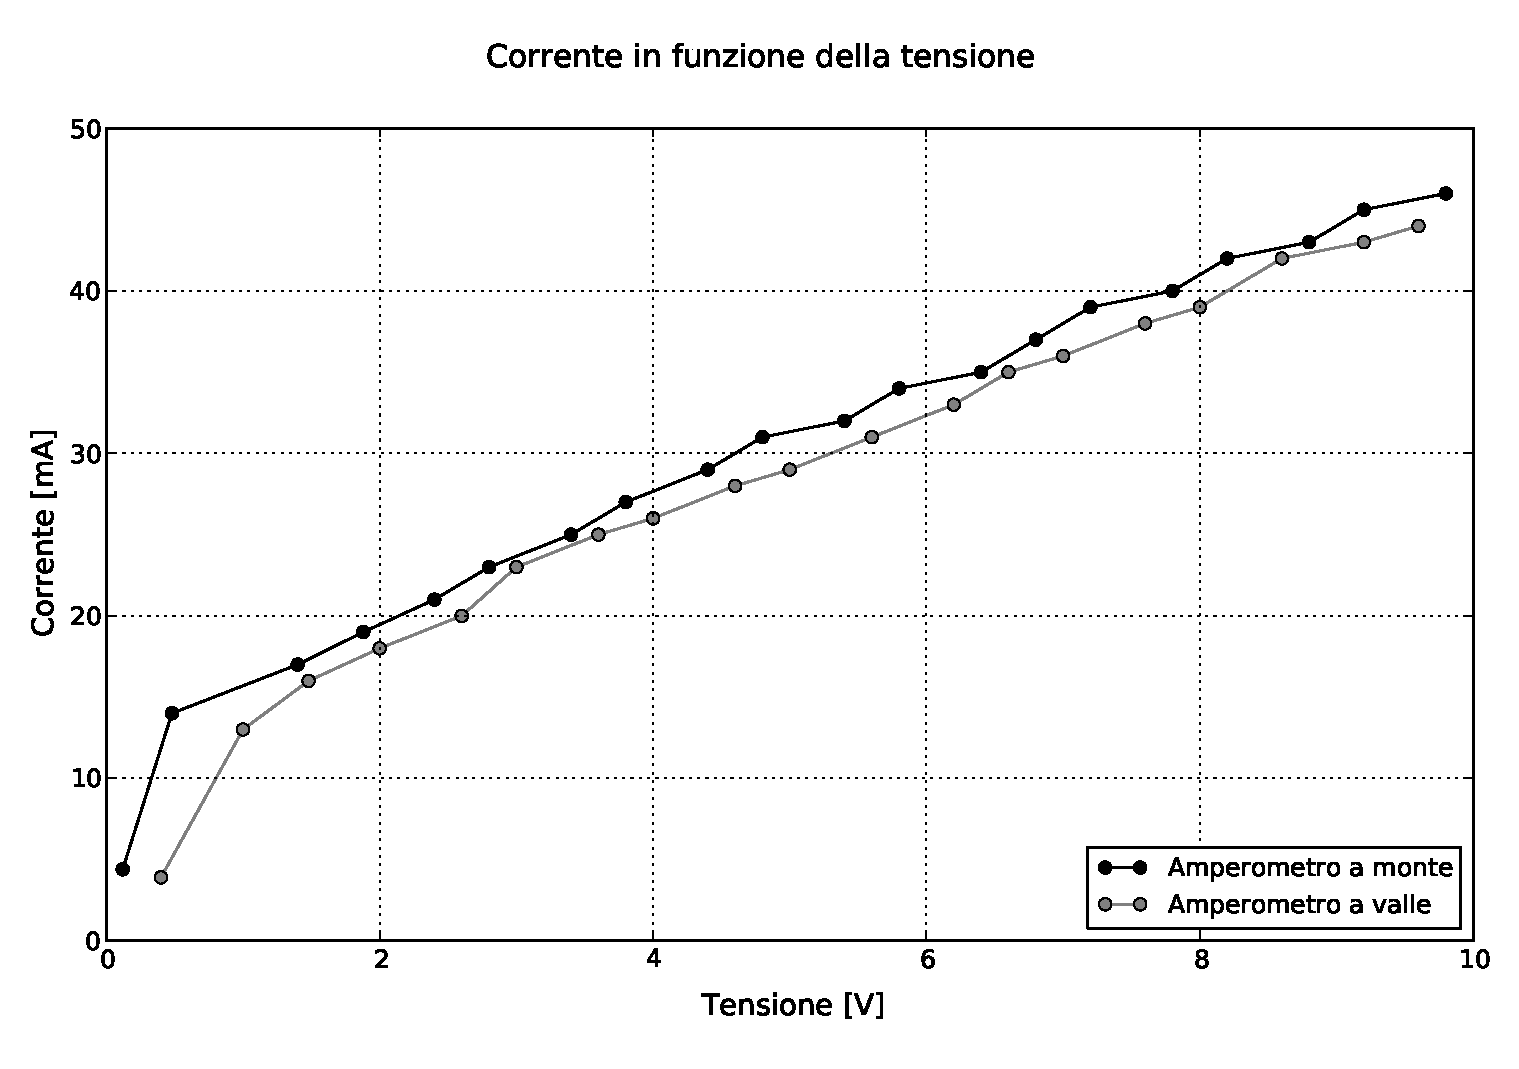
\includegraphics[scale=0.55]{lampadina.pdf}
\end{figure}

